\documentclass{article}
\usepackage{graphicx} 
\usepackage{float}
\usepackage{url}
%\usepackage{hyperref}

\title{LLM-based System for Virtualization of Field Museum's Botanical Collection}
\author{Riley Herbst}
\date{May 7, 2025}

\begin{document}

\maketitle

% -------------------------------------------------
% Abstract
% -------------------------------------------------
\section*{Abstract}
$\quad$ Natural history collections house tens of millions of specimens globally. Millions of those specimens consisting of herbarium sheets whose labels contain taxonomic, geographic and assorted data across 24 fields. Because most of this data exists on handwritten and typed labels, museums still rely on hand transcriptions by humans. Virtualization of the collection by hand is a slow and expensive process. Moreover, human agents are unable to keep pace with virtualization needs. Existing OCR systems have unacceptable error rate on the handwriting recognition, and past vision language models (VLM's) have a set of their own problems. This project takes on the challenge of creating an \textit{almost} fully automated transcription pipeline, complete with image pre-processing, image segmentation, reasoning model text correction and cross validation. Various models were tested including Anthropic's Claude 3.7, OpenAI's GPT 4o, GPT o4-Mini, META's Segment Anything Model (SAM) and Google's Cloud LLM assisted OCR tool. Testing on 260 handwritten and typed labels, the process boosts accuracy  from roughly 60\% of previous pipelines to being in the range between 80\% and 90\% accuracy on exact matches in all categories. The result of pre-processing and combined model approach brings a potential solution for the large scale digitization and transcription that museums across the world need.


% -------------------------------------------------
\section{Introduction}
% -------------------------------------------------


\subsection{ Context of this Study}
$\quad$Over the past year and a half a small team at the Field Museum has been working on a fully automated Image transcription pipeline[1]. In the age of the digital world having constant advancements in technology it was natural to attempt to do this process with Artificial Intelligence (AI). With tens of millions of records still needing to be transcribed AI transcribing systems  has transformed from a novelty experiment to a project spanning many researchers and departments across the world attempting to leverage language models for historical records [2]. With AI technology advancing daily and new models being released it is essential to stay ahead of the curve and harness the power of these models. The introduction of reasoning models have allowed the use of a chain of thought for the transcription process. This iteration on the Field Museum’s work shows the power of image pre-processing and image augmentation models for the advantage of compartmentalizing data to be transcribed. Various models were tested including Anthropic's Claude 3.7[3], OpenAI's GPT 4o, GPT o4-Mini[4], META's Segment Anything Model (SAM)[5] and Google's Cloud LLM assisted OCR tool [6]. With a previous study completed, the goal of this study is to see potential avenues of improving accuracy, speed and reliability of transcription. 

\subsection{Current Transcription Process}
$\quad$The Field Museum has been transcribing images and specimens for years. The use of employees and volunteers has done the work of taking individual specimens, applying barcodes and hand transcribing images into proprietary databases. As well as transcribing, the museum has had a process of photographing specimens in conjunction with a simple OCR tool to start the transcription process. While this process is accurate it has proven to be lengthy. The process of transcribing by hand includes being able to identify a vast amount of information: it is not limited to Who collected a specimen, where it was collected, taxonomic information, observations — and much more. In the past large crowd source programs and out-sourcing have sped up the process. 

\subsection{Past Automated Approach}
$\quad$With the manual process of transcription being subject to human availability, we have tested approaches to fully automated transcription process with minimal user input. The input included only the input of the URL's, a chosen prompt and a model of choice (GPT 4o, Claude 3.5 Sonnet and Google Gemini 1.5 pro). The prompt included a set of instructions and fields with standardized fields (Darwin Core)[7] and consisted of 24 fields. The user would provide a .txt file of a list of URL's, full sized images were sent to their respective models and in time, would be given an output of transcribed labels with information put into specified fields. Issues arose as testing progressed and steps were taken to mitigate said problems. At the time these models were not suited for this application so errors were frequent. Hallucination was a large problem at first, instances of transcriptions having completely unrelated information occurred and were dealt with by prompt engineering and model advancements over time. The combination of handwritten, typed and a mixture of both challenged the models knowledge and algorithms to effectively provide information off the context in the specimens. Hence, testing for the first study was conducted mainly with typed labels. In our testing we brought accuracy up significantly from our firsts tests. 

$\quad$Table 1. shows our preliminary tests were done for image cropping, the idea consisted of hand cropping images from full herbarium sheets to just text dense regions. Results showed significant improvements in field accuracy so the idea and hypothesis of image segmentation was thought of. Tests with cropped images showed promise, hence our segmentation pipeline (1). Shown below is the accuracy jump by using cropped images.

\noindent\textbf{Table 1.} A summary of later findings of image cropping. Results show an increase on all fields when images are cropped to smaller parts, enhancing text clarity and removing distractions from the LLM. Full image overall accuracy shows the results with full herbarium sheets and cropped label overall accuracy shows the cropped label accuracy.[1]

$$
\begin{array}{|l|c|c|}
\hline
\textbf{Field name} & \textbf{Overall accuracy:} & \textbf{Overall accuracy:} \\
                    & \textbf{full image}        & \textbf{cropped label}     \\
\hline
\texttt{collectedBy}           & 64.0\% & 85.0\% \\
\texttt{recordNumber}          & 53.0\% & 74.0\% \\
\texttt{minimumEventDate}      & 69.7\% & 88.9\% \\
\texttt{verbatimIdentification}& 32.0\% & 46.0\% \\
\texttt{latestScientificName}  & 50.0\% & 61.0\% \\
\texttt{identifiedBy}          & 46.8\% & 54.6\% \\
\texttt{firstPoliticalUnit}    & 74.4\% & 83.3\% \\
\texttt{secondPoliticalUnit}   & 32.0\% & 48.0\% \\
\texttt{locality}              & 8.0\%  & 22.0\% \\
\texttt{verbatimCoordinates}   & 8.9\%  & 22.9\% \\
\hline
\end{array}
$$

\subsection{Goals and Proposed Improvements of this Study}
$\quad$With a solid idea of what our goal is and ample testing, new ideas can be explored. The goal of this project is to explore the efficacy of image Pre-Processing before our automated transcription process. Using past data analysis metrics and ideas proposed at the end of our past experiment this new pipeline provides insight as to the efficacy of pre-processing. In this Study I
\begin{enumerate}
\item Continue to use accuracy metrics of LLM-based herbarium label transcription. 
\item Continue to use our previous frameworks and processes to ensure a smooth combination of the two studies.
\item Create a full pre-processing pipeline
\item Utilize LLM assisted OCR for text extraction
\item Utilization of reasoning models for verification of transcripts
\item Keep our goal of having the pipeline be portable and easy to use
\item Use a combined model approach to leverage multiple models
\end{enumerate}
$\quad$The study still uses commercially available LLM's as our main transcription models. The use of open source projects for the process have allowed for costs savings and scalability without the fear of a budget for using these projects. Tests were completed using open-source LLM's (LLama, Qwen) but due to restrictions of hardware being tested on these models were not up to par compared to paid consumer models such as Claude and Chat GPT. As improvements to hardware and models become more accessible our pipeline is flexible enough to allow for new advancements and tests to be completed.  



\section{Methods}


\subsection{Past Work on this Topic}
$\quad$All past work and current project files can be found in the following citation and GitHub links. 

\textbf{Past Paper:} \url{https://www.sciengine.com/DI/doi/10.3724/2096-7004.di.2025.0011}

\textbf{Current Repository:} \url{https://github.com/rherbst123/FieldMuseumTranscription}

\subsubsection*{Software \& Tools}
$\quad$This section contains a list of software, package versions. A list of all prompts, updates and past experiments as well as ground truth for this experiment can be found here: 

\url{https://github.com/rherbst123/RileyHerbstProject}

\subsection{Hypothesis from Past Study}
$\quad$Concluding our past study, there were two major ideas brought up for improvement. Cropped labels and cross validation. With jumps in accuracy shown from image cropping and even greater improvement with cross validation. The thought of image segmentation came to mind and was put into action. Due to its availability and open source nature META's SAM was chosen for our image segmentation model. Cross validation was done using the same process conceived in our past report to ensure consistency in our results. Cross validation is using a combined approach leveraging multiple models. 

\subsection{Dataset}
$\quad$The past study experimented with a range of datasets, eventually landing on a set of 100 types labels. Initially a set of 300 mixed handwritten and typed labels was compiled. This project uses that dataset but eliminates images in that dataset that will not benefit from segmentation. Out of the 300 images 40 of these images were label only images. Due to the nature of the testing of segmentation the 40 label only images were removed. Hence, a dataset of 260 images was created. This dataset was created by experts at the field museum and the full 300 dataset was used extensively in past tests. All images in this dataset have the possibility of being improved and cropped automatically with segmentation. The nature of this dataset is to provide challenges for system validation. A mixture of handwritten and typed text, labels pasted vertically, and damaged or faded text on many of the sheets, let us prepare and test with the most challenging datasets.


\begin{figure}[h!]
  \centering
  \includegraphics[width=.99\linewidth]{Blank diagram (2).jpeg}
  \caption{The Architecture of this system}
  \label{fig:enter-label}
\end{figure}



\subsection{Pipeline Overview}
$\quad$Images are downloaded sequentially using URL's chosen by the user of the program. The URL's are accessed and downloaded with an index to ensure order is kept. 
\begin{enumerate}
\item Each image is firstly placed in a cache folder for safe keeping and to give the option to verify all images are correctly downloaded. 
\item Each image in this folder is then sent through the first pre-processing step, Image Resizing. To ensure all images are standardized each image's dimensions are changed to 1500 X 2250. These images then replace the initial images downloaded. Next, image saturation and brightness are applied as a precursor for segmentation. The goal of using saturation and brightness is to bring out the borders of features on the image. This assists in the segmentation process and some images have high bloom and brightness on images which remove clear borders. Image brightness is 0.9 times the strength of the original and saturation is 1.2 times stronger. These enhanced images are saved to a new folder and a prefix of ``sat\_'' is added to have a clear distinction between before and after. 
\item After Images have been modified segmentation can take place using SAM. The model is called and runs a single image at a time. Masks are created by the model and a new folder with sub folders for each image is created. The number of masks vary per image. After segmentation we are left with a range of 25 to over 100 masks for per image. An IOU score is applied for segmentation for duplicate masks to be eliminated.  Most masks are unimportant and do not contain text. Features range from single leaflets to single words that were segmented out. The goal of segmentation for this process is to isolate the text dense regions of each image. To remove all other unneeded segments a simple OCR is used (EasyOCR). OCR is used in this case to only determine if a segment has text in the image, if text exists in the image it is kept otherwise it is removed from the folder. After this step there still are rogue segments that are unnecessary but still contain text. These segments are removed through a series of tight thresholds that have been tested. 
\item Once all unnecessary segments have been removed only text dense information segments should remain, these segments are the labels, tags and other important information on the specimen voucher. 
\item The remaining segments are collaged into a single image only containing correct segments. 
\item For the first leg on our multi model approach each segment collage per image is sent to OpenAI's GPT 4o for text extraction. The second leg sends a full high resolution image to GPT 4o also, having both of these runs go in parallel ensure that all text is extracted.
\item A third run is started by utilizing Google's OCR. A pass is completed over each individual segment and a text output is created. Each segment has a text output along with each segment. 
\item Next, Claude 3.7 Sonnet is provided the OCR'd text and the segment with the goal of verifying each output from the OCR, the text is then combined with another pass through Claude 3.7 sonnet to compile all of the data into one list of fields. 
\item After all three runs are completed a cross validation script is ran to ensure the models agree on the transcription. Results are compared to the ground truth to get an accurate accuracy score for each field and for overall accuracy. In the end the output from each LLM should look similar in format to the following:
\end{enumerate}

\begingroup
\footnotesize          
\begin{verbatim}
verbatimCollectors: John J. Engel, Matt von Konrat & John E. Braggins
collectedBy: J. Engel
secondaryCollectors: M. von Konrat, J. E. Braggins
recordNumber: 23773
verbatimEventDate: 12 February 2003
minimumEventDate: 2003-02-12
maximumEventDate: 2003-02-12
verbatimIdentification: Telaranea lindenbegii var. papillata Engel & Merr.
latestScientificName: Telaranea lindenbegii var. papillata Engel & Merr.
identifiedBy: J. Engel, M. von Konrat, J. E. Braggins
verbatimDateIdentified: 12 February 2003
associatedTaxa: Blechnum novae-zelandiae, Weinmannia and Dicksonia squarrosa, Leptospermum scoparium
country: New Zealand
firstPoliticalUnit: North Island
secondPoliticalUnit: Auckland Province
municipality: N/A
verbatimLocality: Whareorino Forest, start of track to Leitch's Hut
locality: Whareorino Forest, start of track to Leitch's Hut
habitat: Clay banks
verbatimElevation: 280 m
verbatimCoordinates: 38 24' 5'' S, 174 49' 8'' E
otherCatalogNumbers: 1173554
originalMethod: Handwritten
typeStatus: holotype
\end{verbatim}
\endgroup

\subsubsection*{2.4.1 Image Fetching and Downloading}
$\quad$Using python \texttt{requests} library, user will enter a .txt file of Image URL's from Bryophite Portal Database. \href{https://www.bryophyteportal.org/portal/collections/index.php}{https://www.bryophyteportal.org/portal/collections/index.php}. 

\begin{itemize}
\item Images are downloaded Sequentially and an index is appended to the beginning. EX: \verb|{0023_C473367F.jpg}|
\item Images are saved to a cache folder for safe keeping.
\item Using the \texttt{requests} library in python, we are able to input url's for images to quickly download images.
\end{itemize}

\begingroup\footnotesize
\begin{verbatim}
# Read URLs from file and store them in a list
with open(file_path, 'r') as file:
    urls = file.readlines()
# Download each image, appending an index to maintain order
for index, url in enumerate(urls):
    url = url.strip()  # Remove any extra whitespace
    try:
        response = requests.get(url)
        response.raise_for_status()  # Check if the request was successful
        # Extract image name from URL
        image_name = os.path.basename(url)
        # Modify image name to include index for ordering
        image_name_with_index = f"{index:04d}_{image_name}"
        save_path = os.path.join(save_folder, image_name_with_index)
\end{verbatim}
\endgroup

\subsubsection*{2.4.2 Image Resizing and Enhancement}
$\quad$Due to the nature of the project, segmentation models perform differently based on resolutions. Testing shows that standardizing images to (1500,2250) Pixels for X,Y axis respectively improves speed of segmentation and accuracy of having a good segmentation. This also allows for segments to retain a clear resolution. Secondly, We will apply a slight saturation to Images, we do this with the goal of defining borders on images more clearly. This lets the segmentation model differentiate borders more efficiently and cleanly. 

\paragraph{Resizing Script}
- This script takes downloaded images and resizes them to (1500,2250) and replaces original images. 

\begingroup\footnotesize
\begin{verbatim}
def resize_images(folder_path):
    # Target dimensions
    target_width = 1500
    target_height = 2250
    # Supported image formats
    supported_formats = ['.jpg', '.jpeg', '.png']
    # Iterate through all files in the folder
    for filename in os.listdir(folder_path):
        # Check if file is an image
        if any(filename.lower().endswith(fmt) for fmt in supported_formats):
            # Full path to the image
            image_path = os.path.join(folder_path, filename)
            try:
                # Open the image
                with Image.open(image_path) as img:
                    # Convert to RGB if necessary
                    if img.mode != 'RGB':
                        img = img.convert('RGB')
                    # Resize image
                    resized_img = img.resize((target_width, target_height), Image.Resampling.LANCZOS)
                    # Save the resized image (overwrite original)
                    resized_img.save(image_path, quality=95)
                    print(f"Resized {filename}")
            except Exception as e:
                print(f"Error processing {filename}: {str(e)}")
\end{verbatim}
\endgroup

\paragraph{Saturation and Brightness Script}
$\quad$This script takes each image and applies a slight decrease in brightness and doubles saturation for each image. In testing this has shown to increase differences in colors for the images giving us a cleaner segmentation.

\begingroup\footnotesize
\begin{verbatim}
def adjust_image(image_path, output_path, brightness_factor, saturation_factor):

    image = Image.open(image_path)
    brightness_enhancer = ImageEnhance.Brightness(image)
    image_adjusted_brightness = brightness_enhancer.enhance(brightness_factor)
    saturation_enhancer = ImageEnhance.Color(image_adjusted_brightness)
    final_image = saturation_enhancer.enhance(saturation_factor)
    final_image.save(output_path)

    return final_image

processed_img = adjust_image(

        image_path=input_image_path,
        output_path=output_image_path,
        brightness_factor=0.9,
        saturation_factor=1.2
\end{verbatim}
\endgroup

\subsubsection*{2.4.3 Image Segmentation Using SAM}
$\quad$Using Meta's SAM 1.0 Model (\texttt{sam\_vit\_h\_4b8939}) model. We take pre-processed and enhanced images. SAM is an open-source segmentation model created by META (Facebook) mainly used for video processing but in our case we do this on individual images. 

\paragraph{SAM setup function}

\begingroup\footnotesize
\begin{verbatim}
def initialize_sam():

    sam_checkpoint = "C:\\Users\\riley\\Desktop\\sam_vit_h_4b8939.pth"  
    model_type = "vit_h"
    device = "cuda"
    sam = sam_model_registry[model_type](checkpoint=sam_checkpoint)
    sam.to(device=device)
    return SamAutomaticMaskGenerator(
        sam,
        points_per_side=24,  # Number of points to sample per side of the image
        pred_iou_thresh=0.80,  # Threshold for the predicted Intersection over Union (IoU) score
        stability_score_thresh=0.90,  # Threshold for the stability score of the mask
        crop_n_layers=0,  # Number of layers to crop from the image
        crop_n_points_downscale_factor=0.7,  # Factor to downscale the number of points when cropping
        min_mask_region_area=14500,  # Minimum area (in pixels) for a mask region to be considered valid
)
\end{verbatim}
\endgroup

$\quad$In this script we specify mainly, \texttt{points\_per\_side}, which specifies how many intersections there are on each side for segmentation, the more sides the higher precision for finding smaller nuances in the images. Along with this \texttt{min\_mask\_region\_area} specifies how large our smallest segmentations will be, this adds a first layer of filtering of segments so we do not end up with hundreds of small images. We set our device to Cuda to utilize our onboard GPU, this lets us process images much faster than using a CPU, 7 GB of Video memory is needed for this model so it is relatively lightweight. For Segment duplicate handling an IOU score is implemented using Jaccard index:




% -------------------------------------------------
% IoU definition
% -------------------------------------------------
$$\large IoU (A,B) = \frac{|A \bigcap B|}{|A \bigcup B|}$$
\begin{itemize}
\item With A and B being the two sets of pixels for each mask
\item With $|A \bigcap B|$ Being the overlap of pixels
\item With $|A \bigcup B|$ Being the area covered by one of the masks being compared to
\end{itemize}




\subparagraph*{Segmentation Generation and Saving}
$\quad$After Initialization, we will run each image into the model with the parameters specified in the previous section. 

\begingroup\footnotesize
\begin{verbatim}
def generate_segmentation(image_path, mask_generator):

    image = cv2.imread(image_path)

    if image is None:
        raise ValueError(f"Failed to read image {image_path}")
    max_dimension = 2048
    scale = max_dimension / max(image.shape[:2])

    if scale < 1:
    image = cv2.resize(image, (int(image.shape[1]*scale), int(image.shape[0]*scale)))
    masks = mask_generator.generate(image)
    # Filter out masks that are too big
    image_area = image.shape[0] * image.shape[1]
    max_mask_area = image_area * 0.8  # look at 80% of image are as segments would be too large
    filtered_masks = [mask for mask in masks if mask['area'] < max_mask_area]
    return filtered_masks, image
\end{verbatim}
\endgroup

\begingroup\footnotesize
\begin{verbatim}
def visualize_and_save_segmentation(image, masks, output_folder):

    #plt.figure(figsize=(10, 10))

    plt.imshow(cv2.cvtColor(image, cv2.COLOR_BGR2RGB))  # Correct color display

    for mask in masks:
        mask_image = mask['segmentation']
        plt.contour(mask_image, colors="red")
    plt.axis('off')
    plt.tight_layout()
    output_file = os.path.join(output_folder,                f'{os.path.basename(output_folder)}_segmentation_visualization.png')
    plt.savefig(output_file, bbox_inches='tight', pad_inches=0)
    plt.close()
\end{verbatim}
\endgroup

$\quad$Images are fed sequentially into the model. An added layer of image resizing is added for an extra layer to ensure all images are the same size. Segments are limited to being a max of 80\% of the image. This eliminates segments that take up the entire image. This figure can be changed to ensure that segments are usable and do not require further processing. In the end an image showing the original image with segments shown and all segments are placed into a folder corresponding to each image. On a set of 300 images, determined by hand that 98\% of images had a perfect segmentation. Meaning that all necessary information was extracted from the image and collaged into a compressed image. A simple visual example of a before segmentation and a visualization of segmentation is shown here:

\begin{figure}[h!]
    \centering
    \includegraphics[width=0.99\linewidth]{Pasted image 20250430094245.png}
    \caption{Segmentation Visualization}
    \label{fig:enter-label}
\end{figure}




\subparagraph*{2.4.4 Segment Mask Cleaning and Sorting}
After we segment whole images, there are cases in which we are left with over 50 segments. Some of these segments are specimens, small parts of labels and random color differences in images. What we are after are strictly text dense segments. 
\begin{itemize}
\item Firstly, we use EasyOCR as a first sweep. This eliminates all segments that do NOT contain text. This includes the specimens, color differences, etc. We also have an application specific threshold that if a segment contains less than 3 words we delete the segment.
\item There are still instances in which segments take up most of the page and contain many features, we do not want this. Since we have standardized our images segments. Segments that are larger than 800 pixels wide and 1500 pixels tall are deleted. All necessary segments do not fit into this category as they take up only smaller portions of the page.
\item Once we use an OCR for text identification this leaves us with segments that do contain text. We do want text regions, not all text is necessarily needed for transcription (EX: scale rulers). 
\item Secondly, after we are left with segments that only contain text. We need to remove the unnecessary text segments. The next code block is our means of removing regions that we do not need. The most common segment left behind is the scale ruler. Dealing with this segment is done by determining if a segment has a height or width (if rule is horizontal or vertical) that is 4.7 times the size of the other side. If the image fits this then it is deleted. All necessary blocks of text and labels are mostly equal on all sides.
\end{itemize}

\begingroup\footnotesize
\begin{verbatim}
if word_count < 3:
                print(f"Only {word_count} words detected in {filename}. Deleting...")
                os.remove(file_path)
                continue
            # If the resolution is higher than 2000x2000, delete the image
if width > 800 and height > 1500:
                print(f"Image {filename} has a resolution of {width}x{height}. Deleting...")
                os.remove(file_path)
                continue
            # If the height is 4 times as large as the width, delete the image
if height >= 4.7 * width:
                print(f"Image {filename} has a height {height} that is 4 times as large as its width {width}. Deleting...")
                os.remove(file_path)
                continue
 if width >= 4.7 * height:
                print(f"Image {filename} has a height {width} that is 4 times as large as its width {height}. Deleting...")
                os.remove(file_path)
                continue
            else:
                print(f"{word_count} words detected in {filename}. Keeping the image.")

                kept_images.append(file_path)
\end{verbatim}
\endgroup

$\quad$After and OCR sweep to identify text, a threshold to eliminate large segments and deletion of uneven segments we are left with a 98.3\% perfect segmentation of a batch of 260 images. Segments are collaged together with a black background and saved to a separate folder with the images original name. Below is an example of a segmentation visualization, showing the borders created.





\subsubsection*{2.4.5 Google Cloud OCR and Text Correction}
As a first pass, Google Cloud OCR is used to extract text from each individual segment. 1:1 pairs of text to segments are created. Examples can be found here https://github.com/rherbst123/RileyHerbstProject/tree/main/Hybrid_Pipeline
\begingroup\footnotesize
\begin{verbatim}
def detect_text(path):
    client = vision.ImageAnnotatorClient()
    with io.open(path, 'rb') as image_file:
        content = image_file.read()
    image = vision.Image(content=content)
    response = client.text_detection(image=image)
    texts = response.text_annotations
    
    if response.error.message:
        raise Exception(f'{response.error.message}')
\end{verbatim}
\endgroup

$\quad$After an organized output is created, both the segment and the OCR text is sent to Claude 3.7 sonnet with a prompt. The prompt used in this step is specifying the task of correcting text.  A payload for the API is shown.
\begingroup\footnotesize
\begin{verbatim}
payload = {
                "model": MODEL_NAME,
                "messages": [
                    {
                        "role": "user",
                        "content": [
                            {"type": "image",
                             "source": {"type": "base64", "media_type": image, "data": b64}},
                            {"type": "text",
                             "text": f"{system_prompt}\n\nRaw text:\n{raw_text}"},
                        ],
                   }
                ],
                "max_tokens": 4098,
                "temperature": 0.0,
            }
\end{verbatim}
\endgroup

$\quad$After this step, we are left with one .txt file containing all information from the corrected ocr text. There are multiple lists of information so another pass through Claude 3.7 sonnet combines all the information into the desired formats. 
\begingroup\footnotesize
\begin{verbatim}
payload = {
            "model": MODEL_NAME,
            "messages": [
                {"role": "system", "content": system_prompt},
                {"role": "user",   "content": user_message},
            ],
            "max_tokens_to_sample": 4096,
            "temperature": 0.0,
        }
\end{verbatim}
\endgroup

$\quad$This payload is simply the previous corrected .txt file for each image and a prompt made to parse text into Darwin Core fields (ref) resembling the output shown in 2.4. 

\subsubsection*{2.4.6 Single Image and Collaged Payloads}
$\quad$Similar to the previous payloads, Chat GPT 4o is used with full vouchers and the segmented collages separately with the same prompt with Darwin Core fields used in the previous section 2.4.5. The outputs of these images are formatted as standard.

\subsubsection*{2.4.7 .csv File Conversion}
$\quad$After all outputs are gathered, each .txt file is parsed and converted to a .csv file for further analysis. This standardizes all outputs and allows for data analysis and cross validation to take place. The .csv file is a field for field replication with the images URL and Image name as an identifier. 

\subsubsection*{2.4.6 Cross Validation and Accuracy Assessment}
$\quad$Cross validation and accuracy assessments are completed using previous methods from the past study with the Field Museum. All tools and configurations were created and standardized by Dan Stille. https://github.com/rherbst123/FieldMuseumTranscription/tree/main/DataAnalysis. For histogram displays and mismatch lists find the tools here. https://github.com/rherbst123/RileyHerbstProject/tree/main/DataAnalysis

% -------------------------------------------------
\section{Results}
% -------------------------------------------------
Table 2 shows the results of a series of test from various methods of transcription. Using different models. All tests use the same 260 Full images and their respective modifications to the image. All results shown are the best result in the testing for their respective tests. 

\noindent\textbf{Table 2.} A summary showing progress of results and the advantages of the pipeline. Results from the previous study will be referenced as a previous benchmark. Each reference number will have a specific testing goal, model used, prompt/prompts used for test and overall accuracy. Ref. 3.1 was tested on a set of 100 Typed Only images cropped to labels. All other Tests are completed using 260 mixed typed and handwritten labels. All fields are classified correct if there is an exact match of the transcription and the ground truth. N/A fields are not counted even if correct.

\begin{figure}
    \centering
    \includegraphics[width=1\linewidth]{Pasted image 20250430190901.png}
    
    \label{fig: Results of components of pipeline}
\end{figure}

\subsubsection*{3.1 Previous Work and Benchmarks}
In the past study, prompt engineering and model testing were the main focus. The team was attempting to obtain the best results from a single shot with a single image and a single prompt. Eight prompt iterations were tested and accuracy ranged from 43.3\% to 60\% on single images and prompt. Datasets ranged in size and specifics, all with the goal of improving the prompt and finding ways to improve it. All images tested with were typed labels only. This standardized the results and gave us an easier dataset to work with in the early stages. Comparing the final cross validated results only gives us a hypothesis of the results for this new pipeline. In the time between the last iteration and now models have improved and our dataset has grown by 2.6 times and now is a full mixture of handwritten and typed. 

\subsubsection*{3.2 Full Images Transcriptions}
Branching off section 2.4.2, and to test model improvements. Full pre processed images were run through GPT 4o, a model that has had its knowledge improved since last study. Single resized, saturated and brightness adjusted images were processed. Accuracy was calculated using the system used for previous benchmarks. Compared to previous results, GPT-4o did not improve on image understanding and results were similar to previous observations. Due to the imperfect nature of the segmentation model we had a 98.3\% perfect segmentation rate. While this is percentage seems fine, there is still room for error. The use of the full images comes into play to fill in that 1.7\% of error that happens. This also allows for another angle of interpretation from the model to extract text and to cover the field of "OtherCatalogNumber". Usually, the information needed for "OtherCatalogNumber" is a 7 digit number found in assorted places on the herbarium voucher. Segmentation has proven to be sub-par at segmenting this area of information. Hence the need for a full voucher extraction 
\begin{figure}[h!]
    \centering
    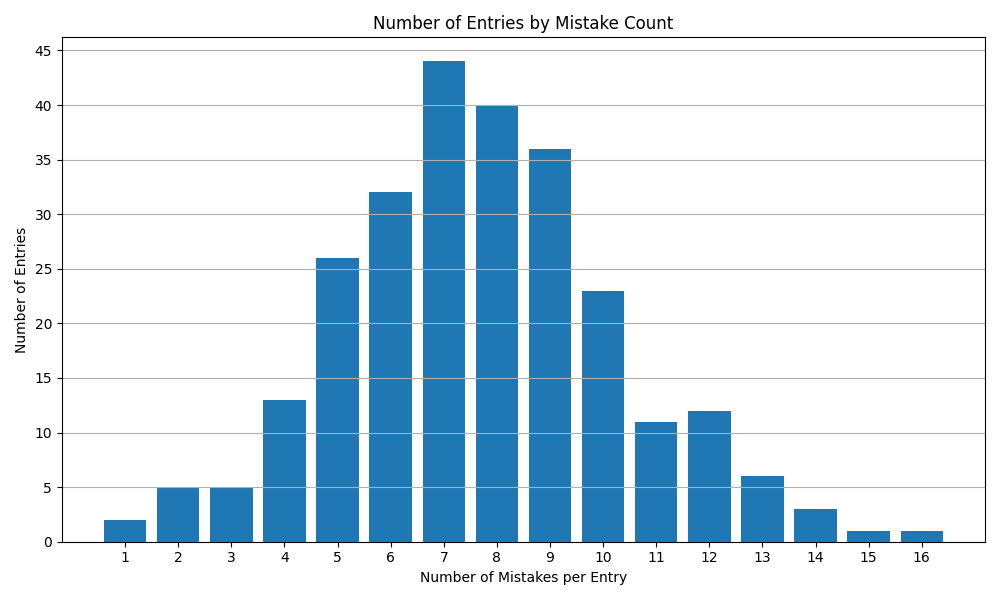
\includegraphics[width=0.75\linewidth]{FullImagesDistribution.png}
    \caption{Full Images Transcriptions}
    \label{fig:enter-label}
\end{figure}



\subsubsection*{3.3 Segmented Collage Transcriptions}
Similar to the previous method, and branching off 2.4.3. A single image of all valid segmentations was sent to the model with a selected prompt. Errors were different from full image transcriptions as the segments at times do not contain all data from the image. We can see this most apparent in the "OtherCatalogNumbers" field. Overall, this process has a slight advantage to the fully transcribed image

\begin{figure}[h!]
    \centering
    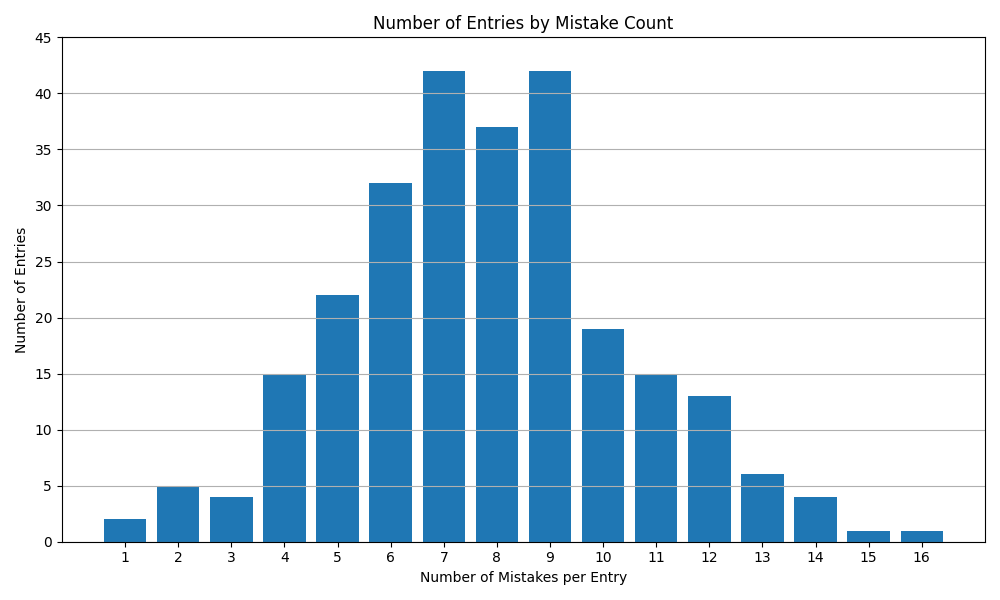
\includegraphics[width=0.75\linewidth]{260Images_4_10_25_Cropped_Full_Images_GPT4o.png}
    \caption{Segmented Collage Transcriptions}
    \label{fig:enter-label}
\end{figure}


$$
\begin{array}{|l|c|c|}
\hline
\text{Field name} & \text{Full-image accuracy} & \text{Cropped-label accuracy} \\
\hline
\texttt{OtherCatalogNumbers} & 64.62\% & 14.62\% \\
\hline
\end{array}
$$


% -------------------------------------------------
\subsubsection*{3.4 OCR Text Correction and Combination}
Straying away from single images and single prompts, reasoning models were brought in to test the use of OCR for a first pass for text extraction. Google Cloud OCR was used to extract text from each segment. During the study it was clear that the OCR had trouble with handwritten text so another pass of LLM viewing the image and OCR text was implemented.

\begin{figure}[H]  % <-- change h! → H
  \centering
  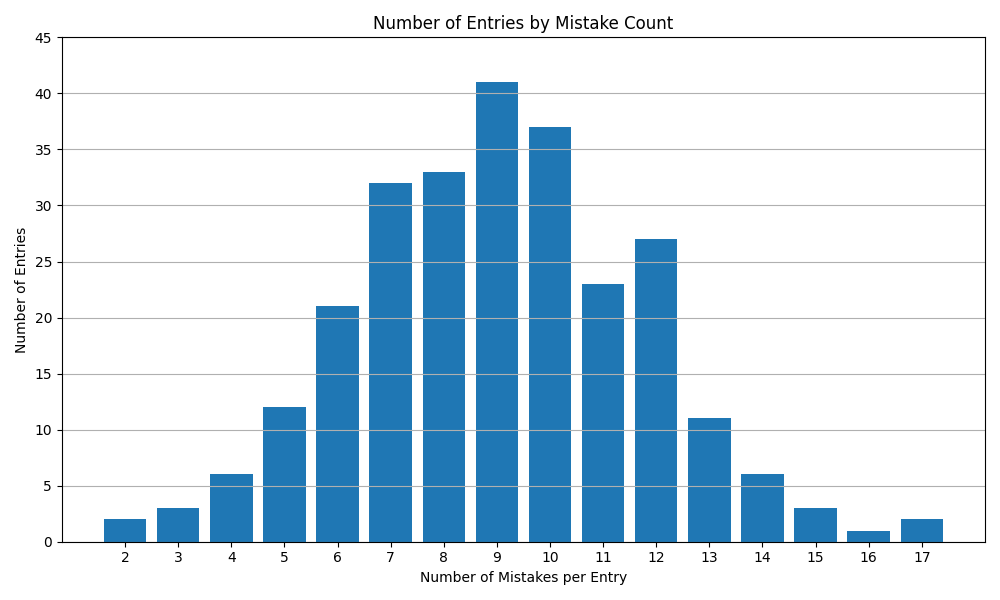
\includegraphics[width=.75\linewidth]{GPT_Corrections_260_Second.png}
  \caption{OCR Text Correction and Combination}
  \label{fig:enter-label}
\end{figure}

\subsubsection*{3.5 Cross Validation}
Combining all three of these perspectives on the image proved to have immense advantages at reasoning with handwritten and mixed text. Our results surpassed smaller and less diverse datasets while remaining similar in time to complete and simplicity. Taking a Full, Cropped and validated image output and combining them limited the errors that each process had while keeping the advantages of each perspective. Compared to results in our past study the results are incremental in some areas but vast in others. The only area of no improvement is in "firstPoliticalUnit". 

\begin{figure}[h!]
    \centering
    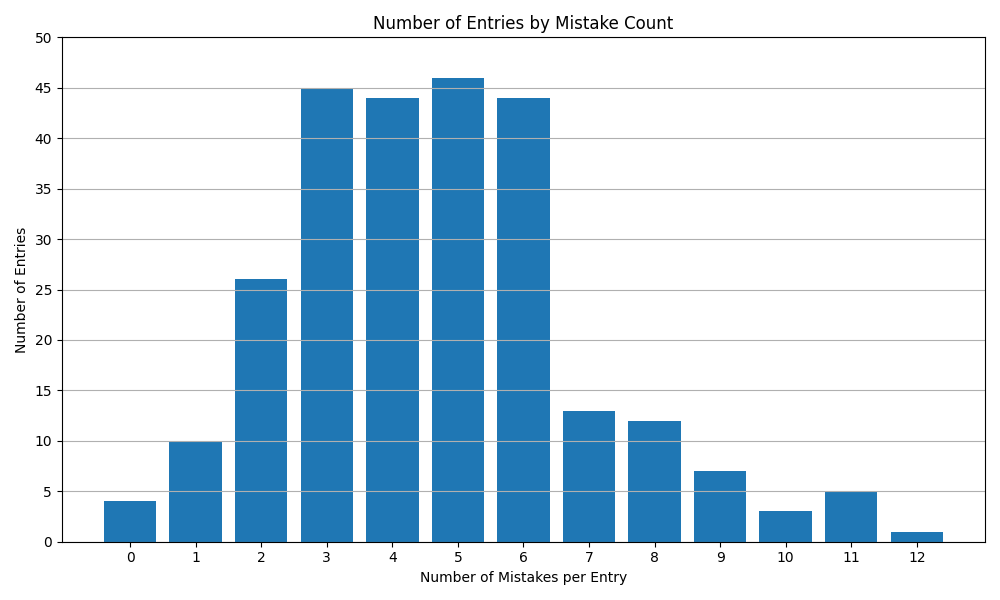
\includegraphics[width=0.75\linewidth]{CrossValidated.png}
    \caption{Cross Validation}
    \label{fig:enter-label}
\end{figure}



$$\small
\begin{array}{|l|c|c|}
\hline
\textbf{Field name} & \textbf{Previous Study} & \textbf{Current Study} \\
\hline
\texttt{collectedBy}           & 85.0\% & 87.3\% \\
\texttt{recordNumber}          & 74.0\% & 92.31\% \\
\texttt{minimumEventDate}      & 88.9\% & 93.0\% \\
\texttt{verbatimIdentification}& 46.0\% & 71.15\% \\
\texttt{latestScientificName}  & 61.0\% & 73.0\% \\
\texttt{identifiedBy}          & 54.6\% & 75.77\% \\
\texttt{firstPoliticalUnit}    & 83.3\% & 79.62\% \\
\texttt{secondPoliticalUnit}   & 48.0\% & 86.54\% \\
\texttt{locality}              & 22.0\% & 25.38\% \\
\texttt{verbatimCoordinates}   & 22.9\% & 89.23\% \\
\hline
\end{array}
$$



\subsubsection*{3.6 Errors}
Similar to the past study, errors came in multiple forms. Errors persisted in the four main categories: transcription errors, logical errors, formatting errors and hallucinations(1). Lists of errors for comparisons can be accessed at: https://github.com/rherbst123/RileyHerbstProject/tree/main/DataAnalysis/Mismatches 

\subsubsection*{3.6.1 Transcription Errors}
Transcription errors consisted of incorrect transcriptions. Usually, a character out of place such as a "u" for an "n" and a "3" for a "5". In the final output for our cross validated transcripts. The recordNumber Field: 

$$\small
\begin{array}{|l|c|c|}
\hline
\textbf{Field name} & \textbf{Ground Truth} & \textbf{Transcribed Label} \\
\hline
\texttt{recordNumber} & 2832 & 2852 \\
\hline
\end{array}
$$
A set of errors that did have some improvement but not impressive results were verbaitmLocality and Locality. Results only rose by 5\% and can in part be attributed to complex unstandardised formats that make exact match transcription extremely difficult. 



\subsubsection*{3.6.2 Logical Errors}
As models have improved, logic errors have reduced. While in past studies there were instances of errors where correct transcriptions were placed in wrong fields. The logical errors in this study consisted of extra data being inserted into fields. For example, with our cross validated result assigned the verbatimCollectors "Amanda Koch Wilson Sakuda AK61 October 22 2003" to the field when the ground truth specified that the correct field value is "Amanda Koch Wilson Sakuda". While the transcription did get the correct spelling and formatting of the name, extra unnecessary data was inserted into the field. 

\subsubsection*{3.6.3 Formatting Errors}
Similar to our past study, many of the mismatches between our output and ground truth were small formatting errors. Many of these errors did not match the prompt or instructions given. Alternatively, due to the nature of human transcription human error is present in parts of the ground truth. Simple mistakes such as formatting inconsistently or improvising formatting during transcription.

$$\small
\begin{array}{|l|c|c|}
\hline
\textbf{Field name} & \textbf{Ground Truth} & \textbf{Transcribed Label} \\
\hline
\texttt{Verbatim Coordinates} & 4^\circ04'N\ 09^\circ02'E & 4^\circ04'N\ 9^\circ02'E \\
\hline
\end{array}
$$

\subsubsection*{3.6.4 Hallucinations}
Hallucinations still persist in this study, but not to the extent of our previous study. Hallucination comes more frequently in with formatting errors and misplacing or adding extra information into specific fields. Capitalization randomly appears through the transcription process despite clear instructions and capitalization not appearing on many of the sheets This error occurs most frequently in  the locality and habitat fields. 

$$\small
\begin{array}{|l|c|c|}
\hline
\textbf{Field name} & \textbf{Ground Truth} & \textbf{Transcribed Label} \\
\hline
\texttt{Verbatim Locality} & Ho\ Volta\ Region\ & HO\ VOLTA\ REGION\ GHANA \\ \hline
\texttt{Habitat} & seaside & Tree\ ca\ 2-3\ m\ tall;\ bark\ with\ light\ blotches;\ flowers\ white \\ 
\hline
\end{array}
$$

% -------------------------------------------------
\section*{4. Discussion and Future Progress}
This branch of our study has explored the advantages of proposed hypothesis from our past study. The use of image segmentation and cross validation were tested and compared, finding specific parameters and models. Image pre-processing, segmentation, collaging, multiple model cross validation were tested. The study obtained multiple insights on the efficacy of these methods. This gave the team insights on what we can keep working on and what to leave out. While problems still occur throughout the process, cross validation has proven to be an effective tool at solving small issues.  

\subsubsection*{4.1 Image Pre-Processing}
Image pre-processing has been the largest focus of this study andhow it affects transcription results. The pre-processing has been compartmentalized into three categories, image resizing, image enhancement and image segmentation. Results varied between each method with image segmentation and text correction proving to be the most effective. With simple image enhancement’s main purpose is to support image segmentation, the results from color enhancement are not too impressive on their own. Results stayed similar to the past study. 

\subsubsection*{4.2 Future Iterations}
As progress is often not linear, there are still challenges to solve. Simple errors such as single character errors or full formatting errors still plague the results. With model improvements releasing constantly and hardware being purchased, the potential increases.ses. One of the most promising techniques yet to be explored is retrieval-augmented generation (RAG). RAG would allow the models to access a knowledge base of information and correct outputs. Depending on its use case, RAG could work as a knowledge base for transcription to have a framework of examples to work from or a validation technique where finished transcriptions are passed through and referenced to correct outputs of the past. Correct names of species, collectors, and updated country names are some of the data that can be inserted into the system to ensure a seamless and cheap way of validating. Open source models have also started to become a more effective and cost conscious way of interacting with LLM's, with many models such as Qwen 2.5-Max and Llama-3.2 Vision proving to be as effective or even more effective in domains than commercially available models such as GPT 4o and Claude

\section*{Conclusion}
This study demonstrates that a pre-processed, almost fully automated built around image pre-processing, image segmentation, and OCR can raise herbarium label transcription rates from a proof of concept to a semi-work ready process. Compared to the previous study (ref paper), the overall field level accuracy climbed from around 60\% to 88\% on a more challenging and larger dataset, containing mixed-typed and handwritten labels. Individual fields such as record Number and verbatim Coordinates achieve the accuracy above 90\%. The largest contributor to the gain was image segmentation: collaging only text dense masks allowed the VLMM to ignore background noise and focus on the pixels most needed. When combined with a second full image pass and OCR + reasoning model, cross validation showed complementary strengths and mostly reduced hallucinations and smaller errors that affected the past study.  


% -------------------------------------------------
\section*{References}
\small
\noindent
[1] R. Herbst \emph{et al.}, “Unlocking the Past: The Potential of Large Language Models to Revolutionize Transcription of Natural History Collections,” \emph{Data Intelligence}, vol.~7, no.~1, pp.~70–94, Feb.~2025, doi: 10.3724/2096-7004.di.2025.0011.\\[0.5em]

[2] M.~P. Polak and D. Morgan, “Leveraging Vision Capabilities of Multimodal LLMs for Automated Data Extraction from Plots,” \emph{arXiv} preprint arXiv:2503.12326, Mar.~2025. \url{https://arxiv.org/abs/2503.12326}\\[0.5em]

[3] Anthropic, “Claude 3.7 Sonnet and Claude Code,” \emph{Anthropic News}, 24~Feb.~2025. [Online]. Available: \url{https://www.anthropic.com/news/claude-3-7-sonnet}. [Accessed: 29-Apr-2025].\\[0.5em]

[4] OpenAI, “Hello GPT-4o,” \emph{OpenAI Blog}, 13~May~2024. [Online]. Available: \url{https://openai.com/index/hello-gpt-4o/}. [Accessed: 29-Apr-2025].\\[0.5em]

[5] A. Kirillov \emph{et al.}, “Segment Anything,” \emph{arXiv} preprint arXiv:2304.02643, Apr.~2023. \url{https://arxiv.org/abs/2304.02643}\\[0.5em]

[6] Google Cloud, “OCR (Optical Character Recognition) | Google Cloud Use Cases,” Google Cloud. [Online]. Available: \url{https://cloud.google.com/use-cases/ocr?hl=en}. [Accessed: 30-Apr-2025].\\[0.5em]

[7] GBIF, “Darwin Core: An Evolving Community-Developed Biodiversity Data Standard,” 2024. [Online]. Available: \url{https://www.gbif.org/darwin-core}. [Accessed: 29-Apr-2025].
% -------------------------------------------------




\end{document}
